% to choose your degree
% please un-comment just one of the following
\documentclass[bsc,twoside,singlespacing,parskip,logo,notimes,normalheadings]{infthesis}
% for BSc, BEng etc.

\usepackage[super]{natbib}
\setcitestyle{square}

\usepackage[absolute,overlay]{textpos}
  \setlength{\TPHorizModule}{1mm}
  \setlength{\TPVertModule}{1mm}

\usepackage{tikz}
\usetikzlibrary{arrows,arrows.meta,decorations.markings}
\usepackage{wrapfig}
\usepackage{amsmath}
\usepackage{caption}
\usepackage{capt-of}
\usepackage{color}
% \documentclass[minf,frontabs,twoside,singlespacing,parskip,deptreport]{infthesis}  % for MInf

\tikzstyle{block} = [rectangle, draw, text width=6em, text centered, rounded corners, minimum height=1em]
\tikzstyle{set} = [rectangle, text width=6em, text centered, rounded corners, minimum height=1em]
\tikzset{vertex/.style = {shape=circle,draw,minimum size=1.5em}}
\tikzset{edge/.style = {
    >=Stealth,
    -{>[scale=1.5]},
  }
}

\newcommand{\cfgpoint}[1][]{%
  \draw[magenta, fill=magenta!90] (#1) circle (0.5mm);
}

\makeatletter
\renewcommand\NAT@citesuper[3]{\ifNAT@swa
\if*#2*\else#2\NAT@spacechar\fi
\unskip\kern\p@\textsuperscript{\NAT@@open#1\if*#3*\else,\NAT@spacechar#3\fi\NAT@@close}%
   \else #1\fi\endgroup}
\makeatother

\begin{document}

\title{Data-Flow Analysis:\\Simulation and Visualisation}

\author{Ayrton Massey}

% to choose your course
% please un-comment just one of the following
%\course{Artificial Intelligence and Computer Science}
%\course{Artificial Intelligence and Software Engineering}
%\course{Artificial Intelligence and Mathematics}
%\course{Artificial Intelligence and Psychology }   
%\course{Artificial Intelligence with Psychology }   
%\course{Linguistics and Artificial Intelligence}    
\course{Computer Science}
%\course{Software Engineering}
%\course{Computer Science and Electronics}    
%\course{Electronics and Software Engineering}    
%\course{Computer Science and Management Science}    
%\course{Computer Science and Mathematics}
%\course{Computer Science and Physics}  
%\course{Computer Science and Statistics}    

% to choose your report type
% please un-comment just one of the following
%\project{Undergraduate Dissertation} % CS&E, E&SE, AI&L
%\project{Undergraduate Thesis} % AI%Psy
\project{4th Year Project Report}

\date{\today}

\abstract{ Data-flow analysis is one of the cornerstones of modern
  compiler optimisation. A thorough understanding of the processes
  involved is essential to further exploration of the subject. A tool
  which allows exploration of data-flow analysis in an interactive
  environment would prove invaluable to students encountering the
  topic for the first time.

  This report describes a interactive system to simulate and visualise
  forms of data-flow analysis on simple assembly-like
  programs. Variations of the system are compared and contrasted by
  exploring user interaction and measuring the achievement of learning
  outcomes of students using this system.  }

\maketitle

\section*{Acknowledgements}
%TODO: Acknowledgements
Acknowledgements go here.

\tableofcontents

%\pagenumbering{arabic}

%%%%%%%%%%%%%%%%%%%%%%%%%%%%%%%%%%%%%%%
\chapter{Introduction}
This chapter gives a short introduction to the topic of data-flow
analysis, describes motivations and desired outcomes for the project
and provides a brief summary of contributions.

    \section{Data-Flow Analysis}
    Data-flow analysis is a tool for analysing the flow of data
    through a program at various points in its execution. Analysis is
    performed over a control-flow graph, computing the properties of
    values flowing {\em in} and {\em out} of each node. Many forms of
    data-flow analysis exist to compute various properties, for
    example {\em liveness analysis} identifies variables which will be
    used in future instructions and {\em available expressions}
    identifies those expressions whose value has been previously
    computed at some point in the control-flow graph.
    
    This analysis is used to inform optimisations which can be
    performed on a given program. Using the example of {\em liveness
      analysis}, the values computed can be used to optimise register
    allocation: a variable which is not live at a given point does not
    need to be allocated to a register, enabling more efficient use of
    available resources.
    
    Data-flow analysis is not only useful in compiler
    optimisation. The information gathered can be used in other ways,
    such as identifying unsafe operations in PHP web
    applications\cite{TaintedFlow} by monitoring sanitization of
    variables which have been assigned to user input.

    \section{Motivations}
    This project was inspired by the project's supervisor, Hugh
    Leather. The original concept was an online tutor for data-flow
    analysis which would allow users to simulate data-flow analysis on
    simple programs. The user could vary parameters, such as the
    data-flow in question or the order in which nodes are evaluated,
    and examine the resulting solution. The system could potentially
    be extended to allow custom data-flows.
    
    As lecturer of the Compiler Optimisations course at the University
    of Edinburgh, Hugh desired a system which could teach students the
    foundations of the course in a more interactive format than
    standard lectures. The system should be suitable for hosting on
    the course web page to make it accessible to all students.
    
    My personal interest in this project stemmed from a desire to use
    my practical skills to increase my capacity for understanding
    theoretical content. As noted in our early discussions, many
    students find it difficult and time consuming to read and
    understand material from the course textbook. Presenting this
    information in such a way that it could be easily digested by even
    a novice to Computer Science provided an exciting challenge.
    
    
    \section{Objectives}
    The main aim of this project was to create an interactive system
    to teach students the basic principles of data-flow analysis in
    compilers.
    
    This would take the form of a web application using modules which
    could be combined in different ways, for example to present a
    series of tutorials on data-flow analysis or to provide a sandbox
    environment to explore. The application would cover a range of
    topics from the basics of data-flow analysis to algorithms and
    frameworks for solving generic data-flow problems.
    
    The application would be aimed at students of the Compiler
    Optimisations course and as such would be based on material from
    the course textbook {\em Engineering a Compiler (2nd Edition)} by
    Keith D. Cooper and Linda Torczon. The application could then be
    extended to cover said material in more depth using content from
    {\em Compilers: Principles, Techniques and Tools, 1st ed.} by
    Alfred V. Aho, Ravi Sethi and Jeffery D. Ullman.
    
    Users would be able to interact with the system by providing
    simple assembly-like programs, altering parameters to the
    simulation and stepping through a simulation. Elements of the
    simulation, such as the current state, would be visualised
    on-screen and update as the simulation progressed. Each of these
    elements would be linked visually to show how the concepts relate.
    
    Variations of the application would be tested on users and
    evaluated in terms of user experience by analysing interactions
    with the system and conducting a user experience
    survey. Achievement of learning outcomes would be assessed by
    examining responses to questions built into the software and
    self-assessment by the user.
    
    \section{Summary of Contributions}
    The final version of the software is capable of the following:
    
    \begin{itemize}
    \item Simulation of pre-defined data-flows using generic framework
      models. (p. )%TODO: Which page?
    \item Simulation of user-defined programs using the
      ILOC\cite[appx.~A]{eac} language from {\em Engineering a
        Compiler}. (p. )%TODO: Which page?
    \item Simulation using the round-robin iterative algorithm (p.
      ) %TODO: Which page?
    \item User-controlled simulation allowing step-by-step, instant or
      automated playback.
    \item Visualisation of the following simulation elements:
      \begin{itemize}
      \item Control-flow graph (p. )%TODO: Which page?
      \item Simulator state incl. currently evaluated node,
        framework etc. (p. )%TODO: Which page?
      \item Table of results displaying data flowing in / out of each
        node
      \item Hasse diagram of meet semi-lattice (p.
        ) %TODO: Which page?
      \end{itemize}
    \item Tutorials covering basics of the topic with interactive
      elements (p. )%TODO: Which page?
    \item Interactive test to assess achievement of learning outcomes
    \end{itemize}

    In addition, I have produced an API to record user interaction
    events modeled on the Google Analytics event model.


%%%%%%%%%%%%%%%%%%%%%%%%%%%%%%%%%%%%%%%
\chapter{Background}
In this chapter I will briefly cover the necessary background
information required to understand this project, both to inform the
reader and to demonstrate my own understanding of the topic.

    \section{Introduction to Data-Flow Analysis}
    Data-flow analysis computes information about data flowing {\em
      in} and {\em out} of each node in a program's control-flow graph
    (or {\em CFG}). Many types of analysis can be performed and the
    information gathered can be used to inform the decisions of
    optimising compilers. A brief list of analyses and their purposes
    can be found in section \ref{analysistypes}.
    
        \subsection{Control-flow Graph}

        \begin{textblock}{80}(20,176)
            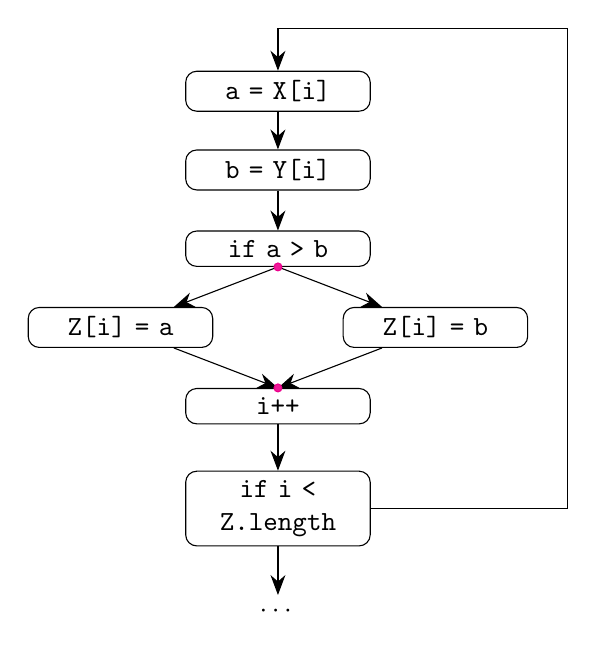
\begin{tikzpicture}[y=-1cm, remember picture]
              % vertices
              \node[block] (n1) at (2 , 0) {\tt a = X[i]};
              \node[block] (n2) at (2 , 1) {\tt b = Y[i]};
              \node[block] (n3) at (2 , 2) {\tt if a > b};
              \node[block] (n4) at (0 , 3) {\tt Z[i] = a};
              \node[block] (n5) at (4 , 3) {\tt Z[i] = b};
              \node[block] (n6) at (2 , 4) {\tt i++};
              \node[block] (n7) at (2 , 5.3) {\tt if i < Z.length};
              \node (n8) at (2 , 6.6) {$\cdots$};
              
              % edges
              \draw[edge] (n1)       to (n2);
              \draw[edge] (n2)       to (n3);
              \draw[edge] (n3.south) to (n4);
              \draw[edge] (n3.south) to (n5);
              \draw[edge] (n4) to (n6.north);
              \draw[edge] (n5) to (n6.north);
              \draw[edge] (n6) to (n7);
              \draw[edge] (n7) to (n8);
              \draw[edge] (n7.east) -| ++(2.5, 0) |- (2.5, -0.8)
              -| (n1.north);

              \cfgpoint[n3.south];
              \cfgpoint[n6.north];
              
            \end{tikzpicture}
            \captionsetup{width=8cm,justification=justified}
            \captionof{figure}{A control-flow graph.}
            \label{cfgexample}
        \end{textblock}

        \hfill\begin{minipage}{\dimexpr\textwidth-6cm}

          A control-flow graph displays the possible execution paths
          for a given program. Each node in the graph represents an
          instruction or basic block, each edge represents an
          execution path leading from that instruction. A node can
          have multiple outward edges if it is a branching
          instruction. Branches may point backward in the
          control-flow. An example of a simple control-flow graph can
          be seen in fig. \ref{cfgexample}.
          
          \vspace{0.26cm}

          A {\em point} in the control-flow graph refers to some point
          along the edges of the graph. In data-flow analysis we
          usually deal with sets of values at the {\em in} and {\em
            out} points of each node, i.e. the point where the {\em
            in-edges} meet and the {\em out-edges} originate,
          respectively (shown in \textcolor{magenta}{magenta} on the
          left).

        \end{minipage}

	\subsection{A Simple Example}
	An oft-used example of data-flow analysis is that of {\em
          reaching definitions}, which we will demonstrate here due to
        its simplicity. Reaching definitions computes the set of
        variable definitions which are are available at a given
        point. A definition is said to {\em reach} a point $p$ if
        there is no intermediate assignment to the same variable along
        the path from the definition of the variable to the point $p$.
        
        Let us take the example in fig. \ref{cfgexample}. The first
        node defines the variable {\tt a}. We shall refer to this
        definition of {\tt a} as {\tt a\textsubscript{1}}. The
        definition of {\tt a} reaches each point in the control-flow
        graph as it is never re-defined. The definition {\tt
          c\textsubscript{1}}, however, does not reach the exit node
        as {\tt c} is re-defined by {\tt c\textsubscript{2}}. The
        graph in fig. \ref{rdcfg} shows the set of reaching
        definitions at each point in the program. We have combined the
        {\em in} and {\em out} points to save space.
        
        \begin{figure}[ht]
          \centering
          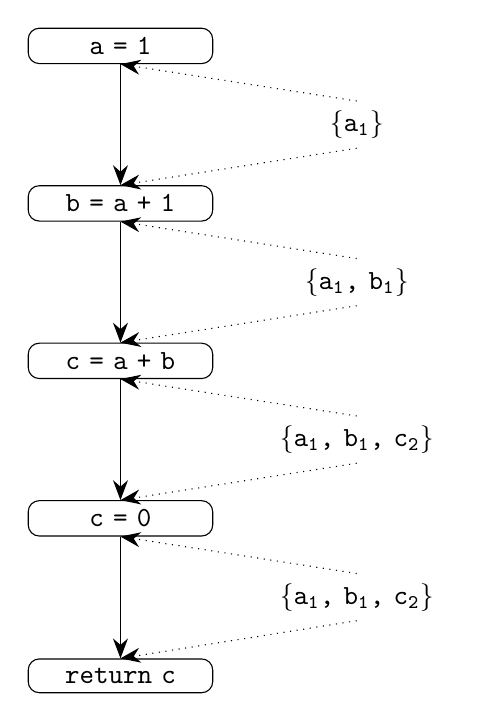
\begin{tikzpicture}[y=-1cm]
            % vertices
            \node[block] (n1) at (0 , 0) {\tt a = 1};
       	    \node[set] (s1) at (3 , 1) {\tt \{a\textsubscript{1}\}};
            \node[block] (n2) at (0 , 2) {\tt b = a + 1};
            \node[set] (s2) at (3 , 3) {\tt \{a\textsubscript{1}, b\textsubscript{1}\}};
            \node[block] (n3) at (0 , 4) {\tt c = a + b};
            \node[set] (s3) at (3 , 5) {\tt \{a\textsubscript{1}, b\textsubscript{1}, c\textsubscript{2}\}};
            \node[block] (n4) at (0 , 6) {\tt c = 0};
            \node[set] (s4) at (3 , 7) {\tt \{a\textsubscript{1}, b\textsubscript{1}, c\textsubscript{2}\}};
            \node[block] (n5) at (0 , 8) {\tt return c};
            
            %edges
            \draw[edge] (n1) to (n2);
            \draw[edge] (n2) to (n3);
            \draw[edge] (n3) to (n4);
            \draw[edge] (n4) to (n5);
            
            %set lines
            \draw[edge, dotted] (s1.north) -- (n1.south);
	    \draw[edge, dotted] (s2.north) -- (n2.south);
	    \draw[edge, dotted] (s3.north) -- (n3.south);
	    \draw[edge, dotted] (s4.north) -- (n4.south);
            \draw[edge, dotted] (s1.south) -- (n2.north);
	    \draw[edge, dotted] (s2.south) -- (n3.north);
	    \draw[edge, dotted] (s3.south) -- (n4.north);
	    \draw[edge, dotted] (s4.south) -- (n5.north);
            
          \end{tikzpicture}
          \caption{A control-flow graph.}
          \label{rdcfg}
        \end{figure}
        
        Data-flows have {\em direction}. Reaching definitions is a
        {\em forward flow problem}; values flow from the entry node of
        the CFG to the exit node.

        The values at each point are determined using {\em data-flow
          equations}. For example, the equations for reaching
        definitions (defined in terms of {\em in} and {\em out}) at a
        given node $n$ are:
        
        \begin{align}
          \textnormal{In}(n)  & = \bigcup_{p \in preds} \textnormal{Out}(n) \\
          \textnormal{Out}(n) & = \textnormal{DefGen}(n) \cup (\textnormal{In}(n) \setminus \textnormal{Out}(n))
        \end{align}
        
        The equations for $\text{In}(n)$ and $\text{Out}(n)$ are often
        referred to as {\em meet} and {\em transfer} (or {\em join})
        functions. In a forward flow problem the meet function
        combines the {\em out} sets of a node's predecessors to form
        its {\em in} set. The transfer function computes a node's {\em
          out} set from its {\em in} set and information obtained from
        the node itself, thereby {\em transferring} values through a
        node.

	\subsection{Lattices}
	Sets in a data-flow problem have a partial order. This can be
        expressed using a structure known as a {\em semi-lattice}. A
        {\em meet} semi-lattice consists of a set of possible values
        $L$, the meet operator $\land$, and a {\em bottom element}
        $\bot$. The semi-lattice imposes an order on values in $L$
        such that:
        
        %TODO: REFERENCE
        \begin{align}
          a \geq b \;\text{if and only if}\; & a \land b = b \\
          a \ge  b \;\text{if and only if}\; & a \land b = b \;\text{and}\; a \neq b
        \end{align}
        
        For the bottom element $\bot$, we have the following:
        
        %TODO: REFERENCE
        \begin{align}
          \forall a \in L,\; & a \geq \bot \\
          \forall a \in L,\; & a \land \bot = \bot
        \end{align}
        
        %TODO: REFERENCE
        We can express the semi-lattice using a {\em hasse diagram}, shown in fig. \ref{meethasse}.

        \begin{figure}[ht]
          \centering
          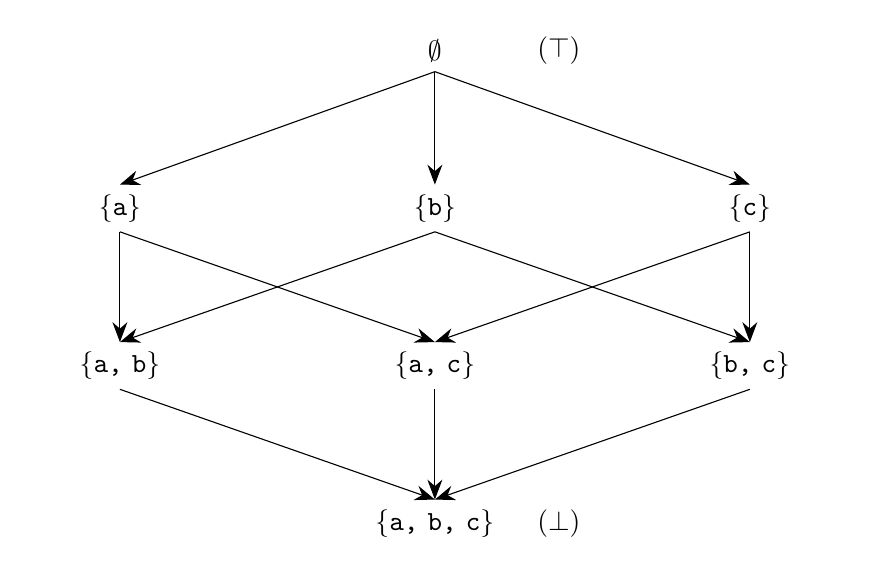
\begin{tikzpicture}[y=-1cm]            
            % vertices
       	    \node[set, label={[distance=1cm]0:$(\top)$}] (s1) at (4 , 0) {$\emptyset$};
	    \node[set] (s2) at (0 , 2) {\tt \{a\}};
            \node[set] (s3) at (4 , 2) {\tt \{b\}};
            \node[set] (s4) at (8 , 2) {\tt \{c\}};
	    \node[set] (s5) at (0 , 4) {\tt \{a, b\}};
	    \node[set] (s6) at (8 , 4) {\tt \{b, c\}};
            \node[set] (s7) at (4 , 4) {\tt \{a, c\}};
	    \node[set, label={[distance=1cm]0:$(\bot)$}] (s8) at (4 , 6) {\tt \{a, b, c\}};
            
            %set lines
            \draw[edge] (s1.south) -- (s2.north);
            \draw[edge] (s1.south) -- (s3.north);
            \draw[edge] (s1.south) -- (s4.north);
            
            \draw[edge] (s2.south) -- (s5.north);
            \draw[edge] (s2.south) -- (s7.north);
            \draw[edge] (s3.south) -- (s5.north);
            \draw[edge] (s3.south) -- (s6.north);
            \draw[edge] (s4.south) -- (s6.north);
            \draw[edge] (s4.south) -- (s7.north);
            
            \draw[edge] (s5.south) -- (s8.north);
            \draw[edge] (s6.south) -- (s8.north);
            \draw[edge] (s7.south) -- (s8.north);
            
          \end{tikzpicture}
          \caption{A hasse diagram for the meet function $a \land b = a \cup b$.}
          \label{meethasse}
        \end{figure}
        
        %TODO: REFERENCE
        Some data-flows deal with sets of pairs of values. In constant
        propagation, we pair a variable with one of three elements:
        $undef (\top)$, $nonconst (\bot)$ and $const$. A variable is
        initially paired with $undef$. When it is assigned a constant
        value, we assign it that value. If it is later assigned
        another value, we assign it $nonconst$. This can be expressed
        as a meet function, seen in fig. \ref{constmeet}.
        
        \begin{figure}[!ht]
        \begin{align}
        nonconst \land c &= nonconst & \text{for any constant} \; c \\
        c \land d &= nonconst &\text{for any constants} \; c \neq d \\
        c \land undef &= c &\text{for any constant} \; c \\
        nonconst \land undef &= nonconst & \\
        x \land x &= x &\text{for any value} \; x
        \end{align}
        \caption{Equations describing the constant propagation meet function.}
        \label{constmeet}
        \end{figure}
        
        These values also form a semi-lattice, seen in fig. \ref{consthasse}.
        
        \begin{figure}[!ht]
          \centering
          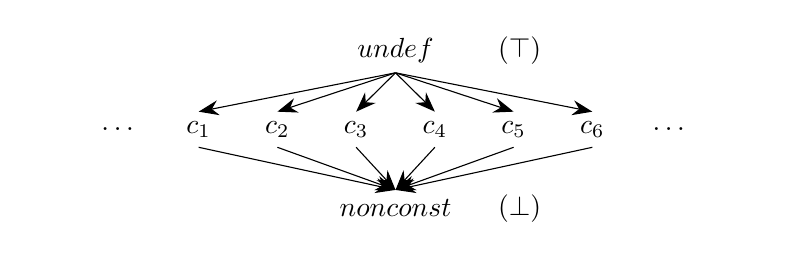
\begin{tikzpicture}[y=-1cm]
            
            % vertices
       	    \node[set, label={[distance=1cm]0:$(\top)$}] (s1) at (3.5 , 0) {$undef$};
            \node[set] (s0) at (0, 1) {$\dots$};
	    \node[set] (s2) at (1 , 1) {$c_1$};
            \node[set] (s3) at (2 , 1) {$c_2$};
            \node[set] (s4) at (3 , 1) {$c_3$};
            \node[set] (s5) at (4 , 1) {$c_4$};
            \node[set] (s6) at (5 , 1) {$c_5$};
       	    \node[set] (s7) at (6, 1) {$c_6$};
            \node[set] (s9) at (7, 1) {$\dots$};
	    \node[set, label={[distance=1cm]0:$(\bot)$}] (s8) at (3.5 , 2) {$nonconst$};
            
            %set lines
            \draw[edge] (s1.south) -- (s2.north);
            \draw[edge] (s1.south) -- (s3.north);
            \draw[edge] (s1.south) -- (s4.north);
            \draw[edge] (s1.south) -- (s5.north);
            \draw[edge] (s1.south) -- (s6.north);
            \draw[edge] (s1.south) -- (s7.north);
            
            \draw[edge] (s2.south) -- (s8.north);
            \draw[edge] (s3.south) -- (s8.north);
            \draw[edge] (s4.south) -- (s8.north);
            \draw[edge] (s5.south) -- (s8.north);
            \draw[edge] (s6.south) -- (s8.north);
            \draw[edge] (s7.south) -- (s8.north);
            
          \end{tikzpicture}
          \caption{A hasse diagram for the meet function described in fig \ref{constmeet}.}
          \label{consthasse}
        \end{figure}
        
        \subsection{Types of Data-Flow Analysis} \label{analysistypes}
        The table in fig. \ref{dfatypes} covers a selection of data-flow analyses and lists some of their applications.
        
        \begin{figure}[!ht]
          \bgroup
          \def\arraystretch{1.5}%
          \begin{tabular}{|l|p{5cm}|p{5cm}|}
            \hline
	        {\bf Data-Flow}                         & {\bf Purpose}                                                                                              & {\bf Applications}                                                                              \\ \hline
                Dominators                              & Computes the set of nodes which dominate the current node.                                                 & Computing SSA form.                                                                             \\ \hline
                Reaching Definitions                    & Computes the set of variable definitions which are available at points in the CFG.                         & Generating def-use chains for other analyses.                                                   \\ \hline
                Liveness Analysis                       & Computes the set of variables whose current value will be used at a later point in the control flow graph. & Register allocation. Identifying useless store operations. Identifying uninitialised variables. \\ \hline
                Available Expressions                   & Identifies expressions which been computed at a previous point in the CFG.                                 & Code motion.                                                                                    \\ \hline
                Anticipable Expressions                 & Computes expressions which will be computed along all paths leading from the current point.                & Code motion.                                                                                    \\ \hline
                Constant Propagation                    & Computes the set of variables which have a constant value based on previous assignments.                   & Constant propagation. Dead code elimination.                                                    \\ \hline
                Copy Propagation                        & Computes the set of variables whose values have been copied from another variable.                         & Dead code elimination. Code motion.                                                             \\ \hline
                Tainted Flow Analysis\cite{TaintedFlow} & Identifies unsafe operations which have been passed unsanitized {\em (tainted)} input.                     & Preventing security vulnerabilities such as SQL injection.                                      \\ \hline
	  \end{tabular}
          \egroup
          \caption{Types of data-flow analysis.}
          \label{dfatypes}
        \end{figure}

	\section{A General Framework}
	Blah Blah
    
    \section{Algorithms for Analysis}
    Blah Blah

	\subsection{Iterative Algorithm}
	Blah Blah

    \section{Intermediate Language for Optimising Compilers}
    Blah Blah


%%%%%%%%%%%%%%%%%%%%%%%%%%%%%%%%%%%%%%%
\chapter{Related Work}
Blah Blah

	\section{Compiler Simulation}
	Blah Blah

	\section{Compiler Visualisation}
	Blah Blah

	\section{Interactive Learning Environments}
	Blah Blah


%%%%%%%%%%%%%%%%%%%%%%%%%%%%%%%%%%%%%%%
\chapter{Data-Flow Analysis Simulation}
Blah Blah

	\section{Data-Flow Framework}
	Blah Blah

        \section{Algorithms for Analysis}
	Blah Blah

	\subsection{Iterative Algorithm}
	Blah Blah
    
    	\subsection{Structural Algorithm}
	Blah Blah
        
	\section{Intermediate Language for Optimising Compilers}
	Blah Blah
    
    	\subsection{Parsing Expression Grammar}
	Blah Blah
    
    	\subsection{Control-Flow Graphs}
        Blah Blah


%%%%%%%%%%%%%%%%%%%%%%%%%%%%%%%%%%%%%%%
\chapter{Data-Flow Analysis Visualisation}
Blah Blah

    \section{Data-Flow Framework}
    Blah Blah
    
    \section{Simulator}
    Blah Blah
    
    \section{Control-Flow Graph}
    Blah Blah
    
    \section{Lattice}
    Blah Blah
    

%%%%%%%%%%%%%%%%%%%%%%%%%%%%%%%%%%%%%%%
\chapter{Interactive Learning}

    \section{User-defined Programs}
    Blah Blah
    
    \section{Interactive Tutorials}
    Blah Blah
    
    \section{Experimental Sandbox}
    Blah Blah
    

%%%%%%%%%%%%%%%%%%%%%%%%%%%%%%%%%%%%%%%
\chapter{Evaluation}
Blah Blah



% use the following and \cite{} as above if you use BibTeX
% otherwise generate bibtem entries
\bibliographystyle{unsrtnat}
\bibliography{mybibfile}

\end{document}